% Try doing this with beamer.

\documentclass{beamer}

\providecommand\insertframetitle{} 

\setbeamertemplate{footline}[page number]
\setbeamertemplate{frametitle}{
\begin{center}
\insertframetitle%
\vspace{-2cm}%
\end{center}
}
\setbeamertemplate{navigation symbols}{}
\setbeamercovered{again covered={\opaqueness<1->{40}}}

\usepackage{graphicx} % To include graphics.

\title{A Search for the Neutrinoless Double Beta
Decay of Xenon-136 with Improved
Sensitivity from Waveform Denoising}

\author{Clayton G. Davis}
\date{April 3, 2014}

\begin{document}

\begin{frame}
\titlepage
\end{frame}

\section*{Outline}
\begin{frame}
\frametitle{Outline}
\tableofcontents
\end{frame}

\section{\texorpdfstring{$\beta\beta 2\nu$ and $\beta\beta 0\nu$}{Two-Neutrino and Neutrinoless Double-Beta} Decay}

\begin{frame}
\begin{center}
\frametitle{What is Double-Beta Decay?}
\end{center}
\begin{columns}
\begin{column}{.5\textwidth}
\includegraphics<1>[keepaspectratio=true,height=180pt]{Avignone_fig02a.eps}
\includegraphics<2>[keepaspectratio=true,height=180pt]{Avignone_fig02b.eps}\\
\tiny Avignone et al., RMP 2008.
\end{column}
\begin{column}{.5\textwidth}
\uncover<1>{Feynman diagram for $\beta\beta 2 \nu$ decay.   Equivalent to two single-$\beta$ decays:
\[ 2n \rightarrow 2p + 2e^- + 2\bar{\nu}_e \]}%
\uncover<2>{Feynman diagram for $\beta\beta 0 \nu$ decay.   Neutrinos annihilate each other:
\[ 2n \rightarrow 2p + 2e^- \phantom{{} + 2\bar{\nu}_e}\]%
$\beta\beta 2 \nu$ is allowed in the Standard Model; $\beta\beta 0 \nu$ is not.}%
\end{column}
\end{columns}
\end{frame}

\begin{frame}
\begin{center}
\frametitle{Implications of Double-Beta Decay}
\end{center}
\begin{columns}
\begin{column}{.5\textwidth}
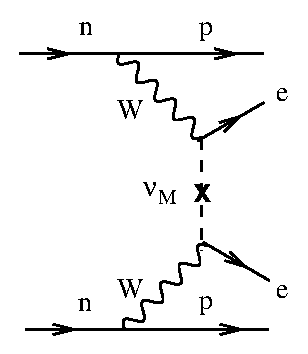
\includegraphics[keepaspectratio=true,height=180pt]{Avignone_fig02b.eps}\\
\tiny Avignone et al., RMP 2008.
\end{column}
\begin{column}{.5\textwidth}
\begin{itemize}
\item Lepton number changes:\[\Delta L = +2\]
\item Neutrinos can convert to their own antiparticle:\[\bar{\nu}_R \rightarrow \nu_L\]
\item Neutrinos have mass through a Majorana interaction:
\[-\frac{m_L}{2}\left(\overline{\Psi^c_L} \Psi_L +  \overline{\Psi_L} \Psi^c_L\right)\]
\[-\frac{m_R}{2}\left(\overline{\Psi^c_R} \Psi_R +  \overline{\Psi_R} \Psi^c_R\right)\]
\end{itemize}
\end{column}
\end{columns}
\end{frame}

\begin{frame}
\begin{center}
\frametitle{The $A=136$ Isobar}
\end{center}
\begin{columns}
\begin{column}{.5\textwidth}
\includegraphics[keepaspectratio=true,width=\textwidth]{LevelDiagram.pdf}\\
\end{column}
\begin{column}{.5\textwidth}
$^{136}$Cs undergoes single-$\beta$ decay.\\[\baselineskip]
$^{136}$Xe cannot, due to energy conservation -- but it can $\beta\beta$ decay through $^{136}$Cs to $^{136}$Ba.\\[\baselineskip]
The $Q$-value of $^{136}\text{Xe}\rightarrow ^{136}\text{Ba}$ is $2457.83 \pm 0.37$ keV, shared between all final products of the decay.\\[\baselineskip]
We observe energy in electrons; energy in neutrinos is lost.
\end{column}
\end{columns}
\end{frame}

\begin{frame}
\begin{center}
\frametitle{Ideal Double-Beta Energy Spectrum}
\end{center}
\includegraphics[keepaspectratio=true,width=\textwidth]{IdealSpectrum.pdf}\\
\only<1>{$^{136}$Xe $\beta\beta 2\nu$ produces a smooth energy spectrum; ``missing'' energy carried off by neutrinos.}
\only<2>{$^{136}$Xe $\beta\beta 0\nu$ has no neutrinos, so no ``missing'' energy; mono-energetic peak at $Q = 2458$ keV.}
\only<3>{If the $\beta\beta 0\nu$ peak exists, neutrinos have Majorana mass; peak height gives a measurement of that mass.}
\end{frame}

\section{The EXO-200 Detector}

\begin{frame}
\begin{center}
\frametitle{The EXO-200 Detector}
\end{center}
\includegraphics[keepaspectratio=true,width=\textwidth]{cleanroom.pdf}
\end{frame}

\begin{frame}
\begin{center}
\frametitle{The EXO-200 Detector}
\end{center}
\begin{columns}[onlytextwidth]
\begin{column}{.5\textwidth}
\includegraphics[keepaspectratio=true,width=\textwidth]{cleanroom.pdf}\\
To search for rare decays, low background is key:
\begin{itemize}
\item Clean (low-radioactivity) materials surrounding TPC.
\item Deep underground to avoid cosmogenics.
\end{itemize}
\end{column}
\begin{column}{.5\textwidth}
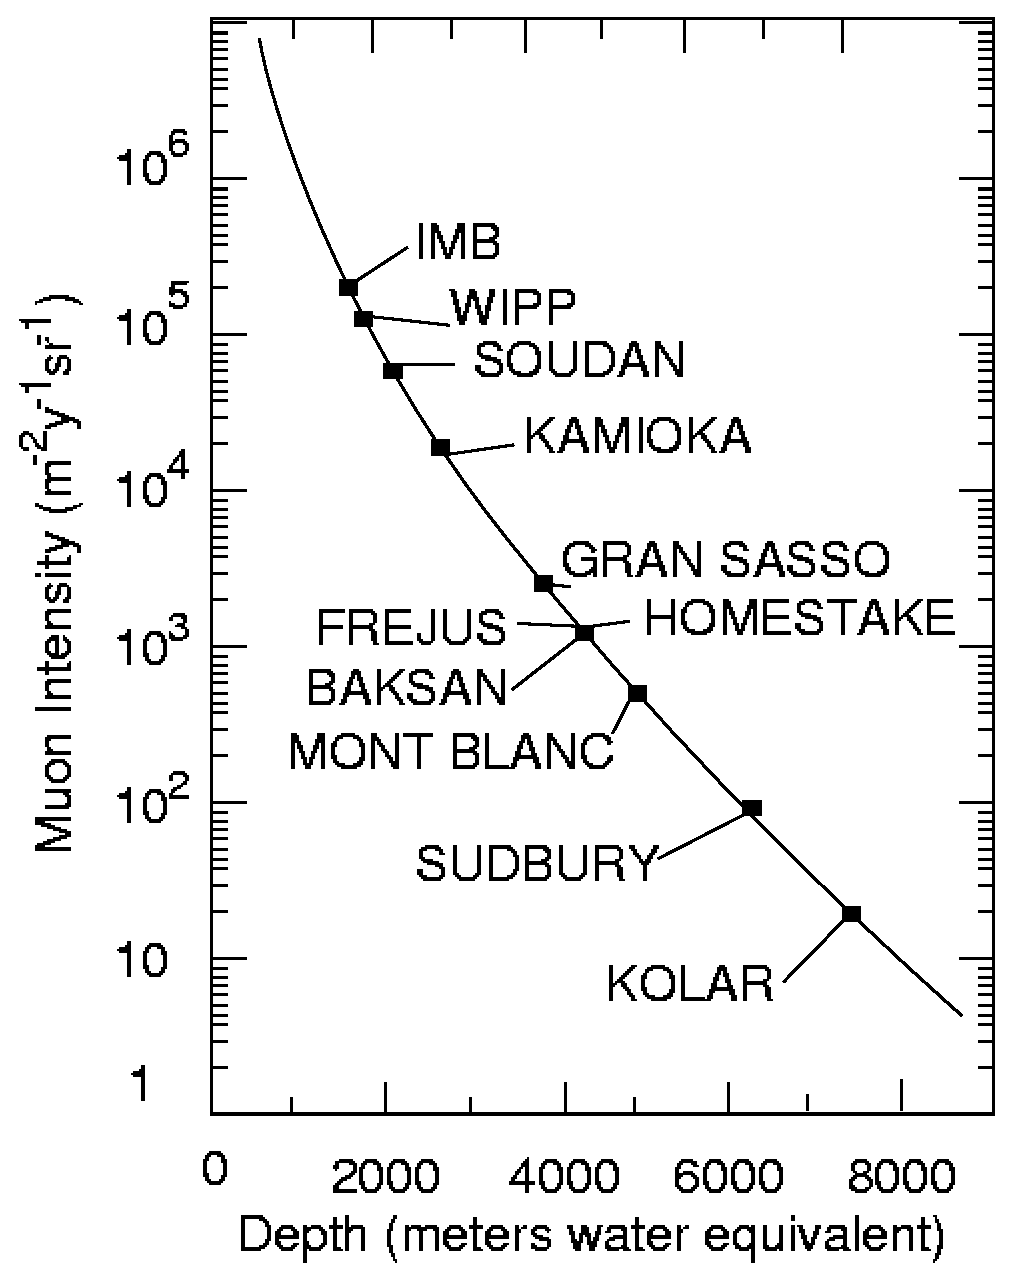
\includegraphics[keepaspectratio=true,width=\textwidth]{muonflux.eps}\\
\tiny Esch et al., NIM A 2005.
\end{column}
\end{columns}
\end{frame}

\begin{frame}
\begin{center}
\frametitle{EXO-200 TPC}
\end{center}
\vspace{1cm}
\begin{columns}[onlytextwidth]
\begin{column}{.25\textwidth}
110 kg of liquid xenon in active volume, enriched to 80.6\% in $^{136}$Xe, contained in a time projection chamber (TPC).\\[\baselineskip]
Xenon continuously circulates through purifiers outside of the cryostat.
\end{column}
\begin{column}{.75\textwidth}
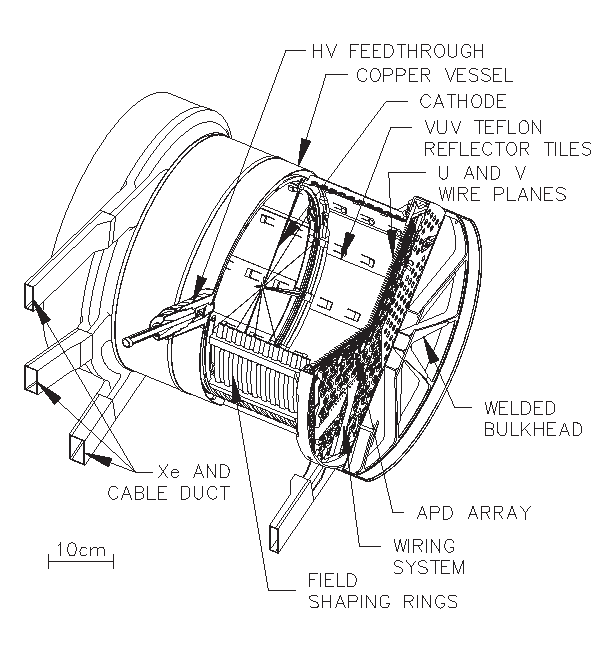
\includegraphics[keepaspectratio=true,width=\textwidth]{TPCSchematic.eps}
\end{column}
\end{columns}
\end{frame}

\begin{frame}
\begin{center}
\frametitle{EXO-200 TPC}
\end{center}
\vspace{1cm}
\begin{center}
\includegraphics[keepaspectratio=true,width=.8\textwidth]{ChargeDrift2DModel.png}
\end{center}
Charge drifts under an electric field and is collected by wires on the anodes.  Light is observed by APDs behind the wires.
\end{frame}

\begin{frame}
\begin{center}
\frametitle{Energy from Ionization and Scintillation}
\end{center}
\begin{columns}
\begin{column}{.75\textwidth}
\includegraphics[keepaspectratio=true,width=\textwidth]{RotationTh2D_withCalibration.pdf}
\end{column}
\begin{column}{.25\textwidth}
Energy is independently measured from scintillation and ionization.\\[\baselineskip]

They are anticorrelated -- better energy resolution from both together than either independently.
\end{column}
\end{columns}
\end{frame}

\begin{frame}
\begin{center}
\frametitle{Primary Backgrounds: $^{232}$Th, $^{238}$U, and $^{137}$Xe}
\end{center}
Here I would show the three plots (with a dashed line to indicate Q-value):
\begin{itemize}
\item Thorium spectrum (SS and MS together)
\item U spectrum (SS and MS together)
\item Xe-137 spectrum (SS and MS together)
\end{itemize}
My concern is that maybe it's better if I don't mention SS and MS discrimination.  It's important, but it's not critical to my main point about the impact of denoising.  But if I have time or if it's critical, I can go back -- so hold off on making these plots.
\end{frame}

\begin{frame}
\begin{center}
\frametitle{Primary Backgrounds: $^{232}$Th, $^{238}$U, and \textcolor{red}{$^{137}$Xe}}
\end{center}
Show plot of Xe-137 first -- smooth background, smooth change in background vs energy resolution.
\end{frame}

\begin{frame}
\begin{center}
\frametitle{Primary Backgrounds: \textcolor{red}{$^{232}$Th}, $^{238}$U, and $^{137}$Xe}
\end{center}
\begin{columns}
\begin{column}{.6\textwidth}
\includegraphics[keepaspectratio=true,width=\textwidth]{Th_Spectra_vs_Res.pdf}
\end{column}
\begin{column}{.4\textwidth}
Description here.
\end{column}
\end{columns}
\end{frame}

\begin{frame}
\begin{center}
\frametitle{Primary Backgrounds: $^{232}$Th, \textcolor{red}{$^{238}$U}, and $^{137}$Xe}
\end{center}
\begin{columns}
\begin{column}{.6\textwidth}
\includegraphics[keepaspectratio=true,width=\textwidth]{U_Spectra_vs_Res.pdf}
\end{column}
\begin{column}{.4\textwidth}
Description here.
\end{column}
\end{columns}
\end{frame}

\begin{frame}
\begin{center}
\frametitle{Backgrounds vs. Resolution}
\end{center}
\vspace{1cm}
\includegraphics[keepaspectratio=true,width=\textwidth]{BackgroundsVsRes.pdf}
\end{frame}


% Plots showing how background decreases with resolution

%%%%%%%%%%%%%%%%%%%%%%%%%%%%%%%%%%%%%%%%%%%%%%%%%%%%%%%%%%%%%%%%%%%%%%%%%%%%%%%

\begin{frame}
\frametitle{Backup Slides}
\end{frame}

\begin{frame}
\begin{center}
\frametitle{Anticorrelated Scintillation/Charge}
\end{center}
\vspace{.5cm}
\begin{center}
\includegraphics[keepaspectratio=true,width=\textwidth]{RotatedIsland.png}
\end{center}
\end{frame}

% X-ray attenuation
% SS/MS (If I don't address it directly.)
% Alpha discrimination.
% Muon-vetoed spectrum.


\end{document}

